\documentclass[a4paper,10pt]{report}
\usepackage[utf8]{inputenc}
\usepackage{hyperref}
\usepackage{graphicx}
\usepackage{float}
% Title Page
\title{Analyse de Comportements avec Twitter}
\author{Antonin Durey Matthieu Caron}




\begin{document}
\pagenumbering{alph}
\maketitle
\clearpage
\pagenumbering{arabic}
\chapter{Description générale du projet}
  \section{Lien vers le git}
    \url{https://github.com/Grimnack/pje2}
  \section{Description de la problématique}
    Le but est de créer une application permettant de tester différents algorithmes
    afin de faire une analyse de sentiments sur Twitter. La problématique est donc la suivante :
    quel est l'algorithme le plus efficace, c'est à dire qui donne le plus souvent la vérité, pour faire de la 
    classification de sentiments ?
  \section{Description générale de l'architecture de votre application}
    Nous avons fait une application Java Swing. Ainsi, nous avons privilégié une architecture MVC.
    Les modèles contiennent les différentes informations permettant à l'application de fonctionner : les éléments graphiques, les tweets, les éléments de configuration...
    Les vues sont représentés par les différents éléments graphiques de l'application.
    Le contrôle est principalement effectué par la classe Annotation qui s'occupe de classer les tweets en fonction de l'algorithme choisi. 
\chapter{Détails des différents travaux réalisés}
  Le projet se divise en quatre tâches majeures : 
  \begin{itemize}
   \item utilisation d'une API twitter afin de récupérer des tweets
   \item préparation une base afin de classifier les tweets selon un algorithme utilisant des techniques d'apprentissage supervisé
   \item implémenter et tester différents algorithmes de classification
   \item se servir de l'application depuis une interface graphique
  \end{itemize}
  \section{API Twitter}
  % image de l'interface graphique et explication
  \section{Préparation de la base d'apprentissage}
    \subsection{Nettoyage des données}
      Pour nettoyer nos données, nous avons effectué les opérations suivantes : 
      \begin{itemize}
       \item Pour les doublons, nous vérifions que les tweets ne sont pas présents en double. Néanmoins, nous considérons qu'un retweet n'est pas un doublon car c'est une manière d'exprimer le même avis que la personne ayant initialement tweeté.
       \item Une option de l'API permet de sélectionner une langue pour les tweets - option que nous avons activé pour s'assurer de ne récupérer que des tweets français.
       \item Nous avons fait un filtrage pour retirer tous les symboles de ponctuation, "RT" signifiant retweet, URL et l'url associée.
      \end{itemize}
      Ce nettoyage comporte plusieurs problèmes. Ne pas considérer que les retweets sont des doublons peut s'avérer problématique.
      De plus, retirer tous les symboles de ponctuation est très risqué quant à l'interprétation de certaines données.
      Par exemple, \textit{11.5Mds} devient \textit{115Mds} après avoir appliqué le filtre.
      

    \subsection{Construction de la base}
      Pour construire notre base de tweets, nous le faisons directement depuis notre application. Nous récupèrons un nombre de tweet paramétrable.
      En cliquant sur \emph{Etiquetage}, il est par la suite possible d'affecter une classe à un tweet.
      Enfin, la sauvegarde dans un fichier permet de créer une nouvelle base, ou d'ajouter des tweets dans une base.

  \section{Algorithme de classification}
    Pour tester les différents algorithmes nous avons d'une part regardé s'il y a une forte différence entre la classe qu'un humain affecterait à un tweet et ce que trouve l'algorithme.
    D'autre part, nous avons analysé le temps de calcul. Nous avons en effet pensé que c'était un facteur très important dans le domaine de la bigdata, même si avions peu de données.
     
    \subsection{mots clefs}
      L'algorithme des mots clefs, ou l'algorithme du dictionnaire, est un algorithme permettant de classer des tweets en fonction d'un dictionnaire établi à l'avance.
      Ainsi, notre application possède un ficher contenant des mots considérés comme positif, et un fichier contenant des mots considérés comme négatifs.
      L'algorithme se contente de regarder combien de mots positifs et négatifs sont présents dans le tweet.
      \begin{itemize}
       \item Si le nombre de mots positifs présents est supérieur au nombre de mots négatifs, le tweet est positif.
       \item Si le nombre de mots positifs présents est inféieur au nombre de mots négatifs, le tweet est négatif.
       \item S'il y a autant de mots positifs que négatifs présents dans le tweet, celui-ci est neutre.
      \end{itemize}

    \subsection{KNN}
      KNN est un algorithme fonctionnant avec une base d'apprentissage.
      
    \subsection{Bayes}
      Bayes a été utilisé dans notre programme pour nous permettre d'estimer la classe des tweets qui vont être ajoutés dans notre base. Ainsi, si l'algorithme de Bayes est bien implémenté et qu'il y a une base conséquence de données, il devient possible d'inclure des tweets dans la base grâce à cet algorithme.
      Néanmoins, il est difficile pour un algorithme d'estimer la classe d'un tweets seulement en regardant mot après mot. C'est pourquoi nous avons ajouté plusieurs paramètres dans notre application :
      \begin{itemize}
	    \item Il est possible d'exclure les mots de moins de n lettres - n étant configurable. Cela permet de ne pas prendre en compte les petits comme les articles, pronoms ou déterminants qui n'offrent que peu de sens et qui ne sont généralement pas significatifs pour classifier un tweet. 
	    \item En prenant un thème donné - la SNCF -, il est logique que certains mots ou groupe de mots soient très important pour juger de la classe d'un tweet. Dans le cas de la SNCF, des ensembles de mots tels que \textit{en retard, à l'heure, train annulé...} sont importants et doivent être davantage pris en compte. Dans l'application, cela est représenté par les \textit{n-grammes}.
      \end{itemize}
      De plus, nous laissons le choix de lancer l'algorithme de Bayes en comptant les mots selon leur présence ou selon leur fréquence.
      Nous nous en sommes rendus compte par la suite : dans le cas d'un tweet où le nombre de mots est réduit, ce changement n'apporte pas beaucoup de différence.
      
      %analyse de Bayes
      
      La vérification de la base consiste à découper la base en n parties - dans notre application, n est égale à 10.
      Elle permet par la suite d'utiliser l'algorithme de Bayes sur chacun des 10 parties de la base en prenant comme base les 9 autres parties de l'ancienne base.
      Cela permet de regarder si la base est cohérente et suffisamment peuplé pour que l'algorithme de Bayes trouve la même classe pour de nombreux tweets de la base.
      Dans notre application, la vérification de la base est implémentée mais ne fonctionne pas.

  \section{Interface graphique}
    \subsection{copie d'ecran}
      \begin{figure}[H]
	\centering
	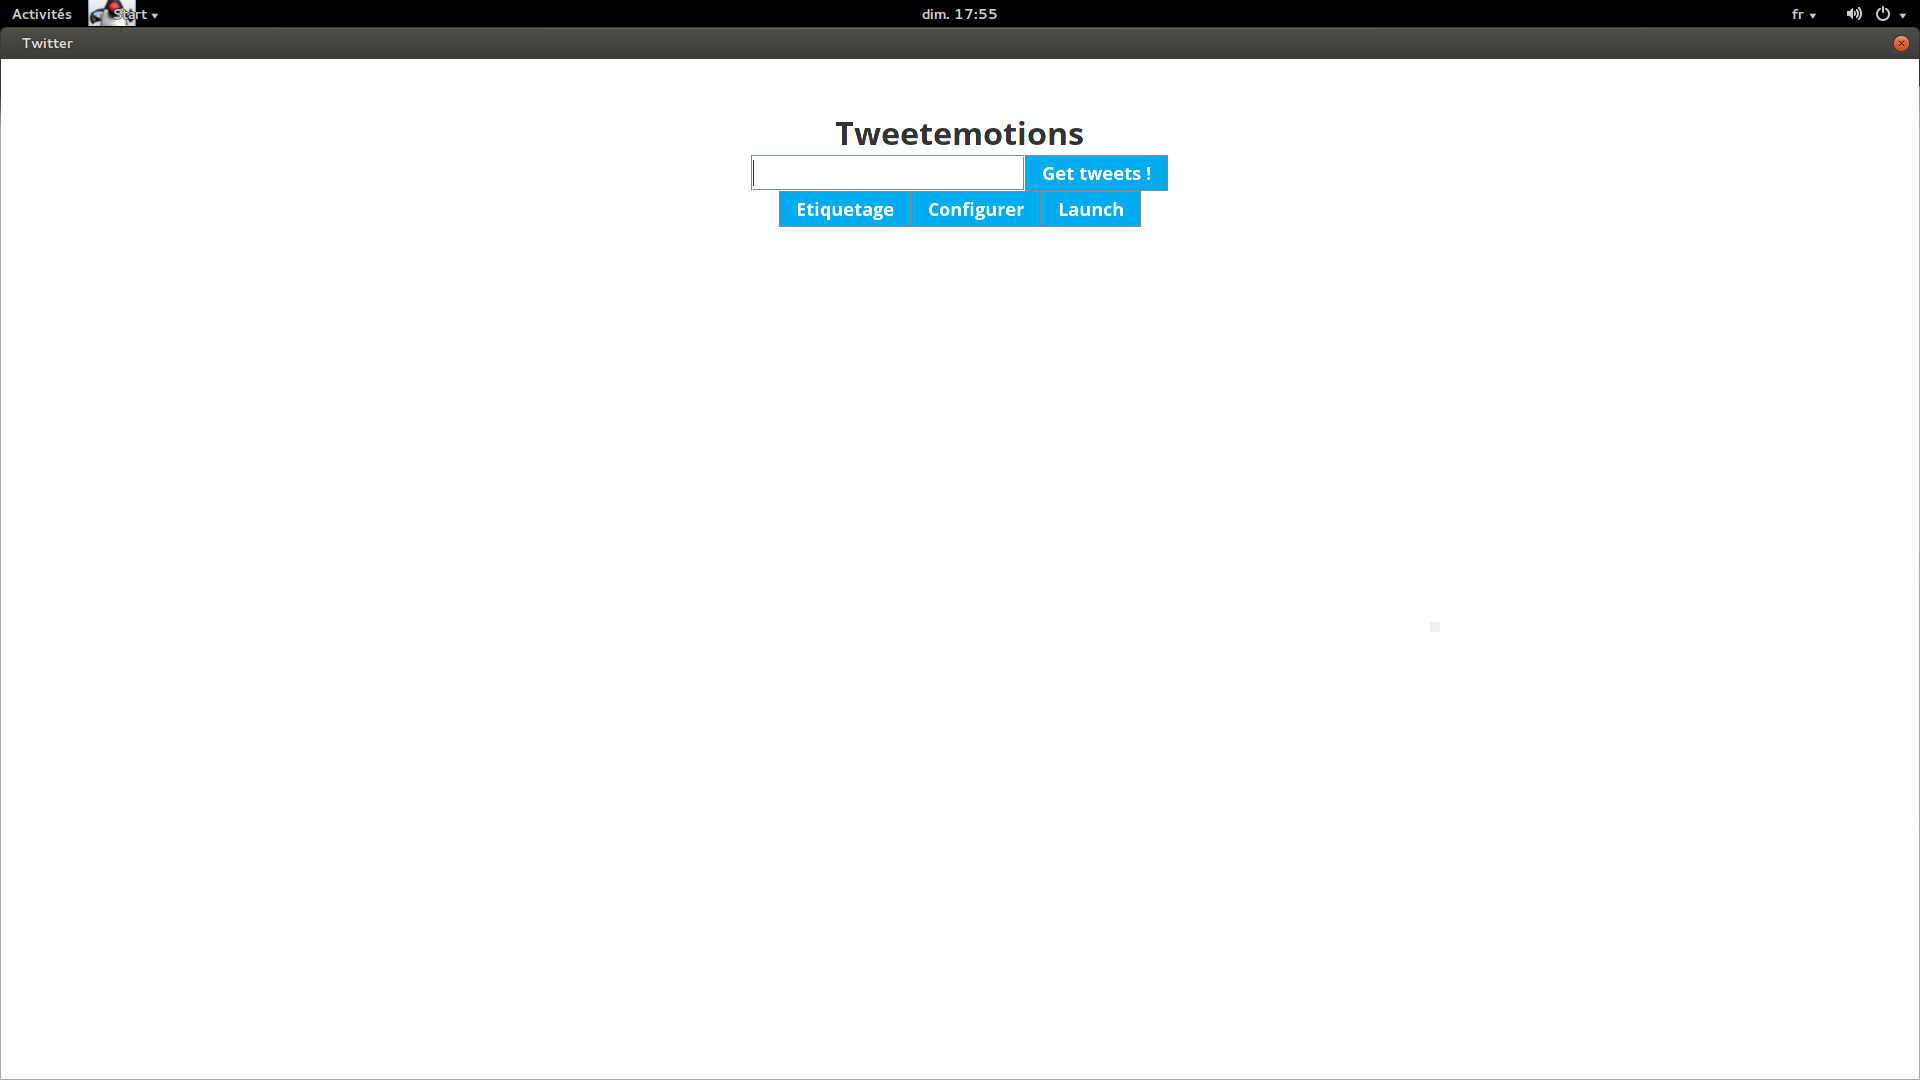
\includegraphics[scale=0.2]{impressions-ecran/accueil.png}
	\caption{Page d'accueil}
	\label{accueil}
      \end{figure}
      \begin{figure}[H]
	\centering
	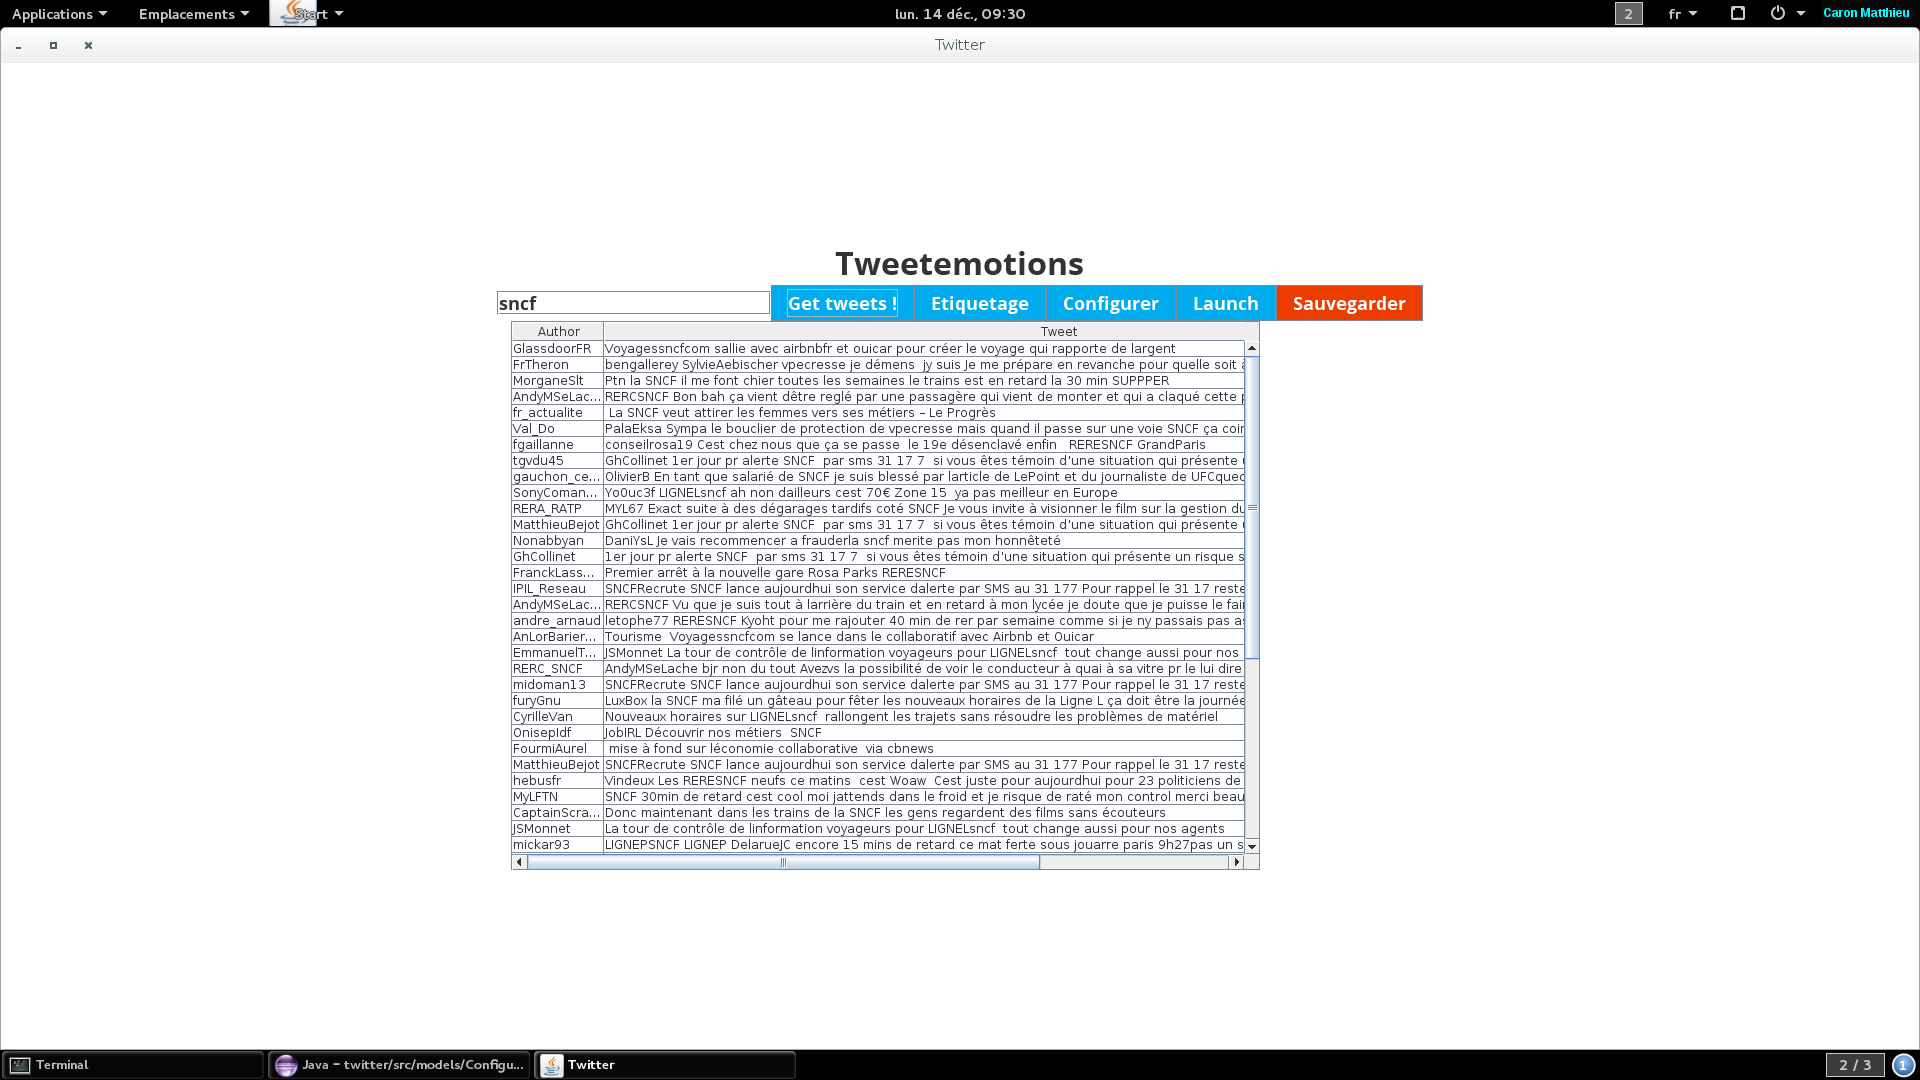
\includegraphics[scale=0.2]{impressions-ecran/tweets.png}
	\caption{Affichage des tweets}
	\label{tweets}
      \end{figure}
      \begin{figure}[H]
	\centering
	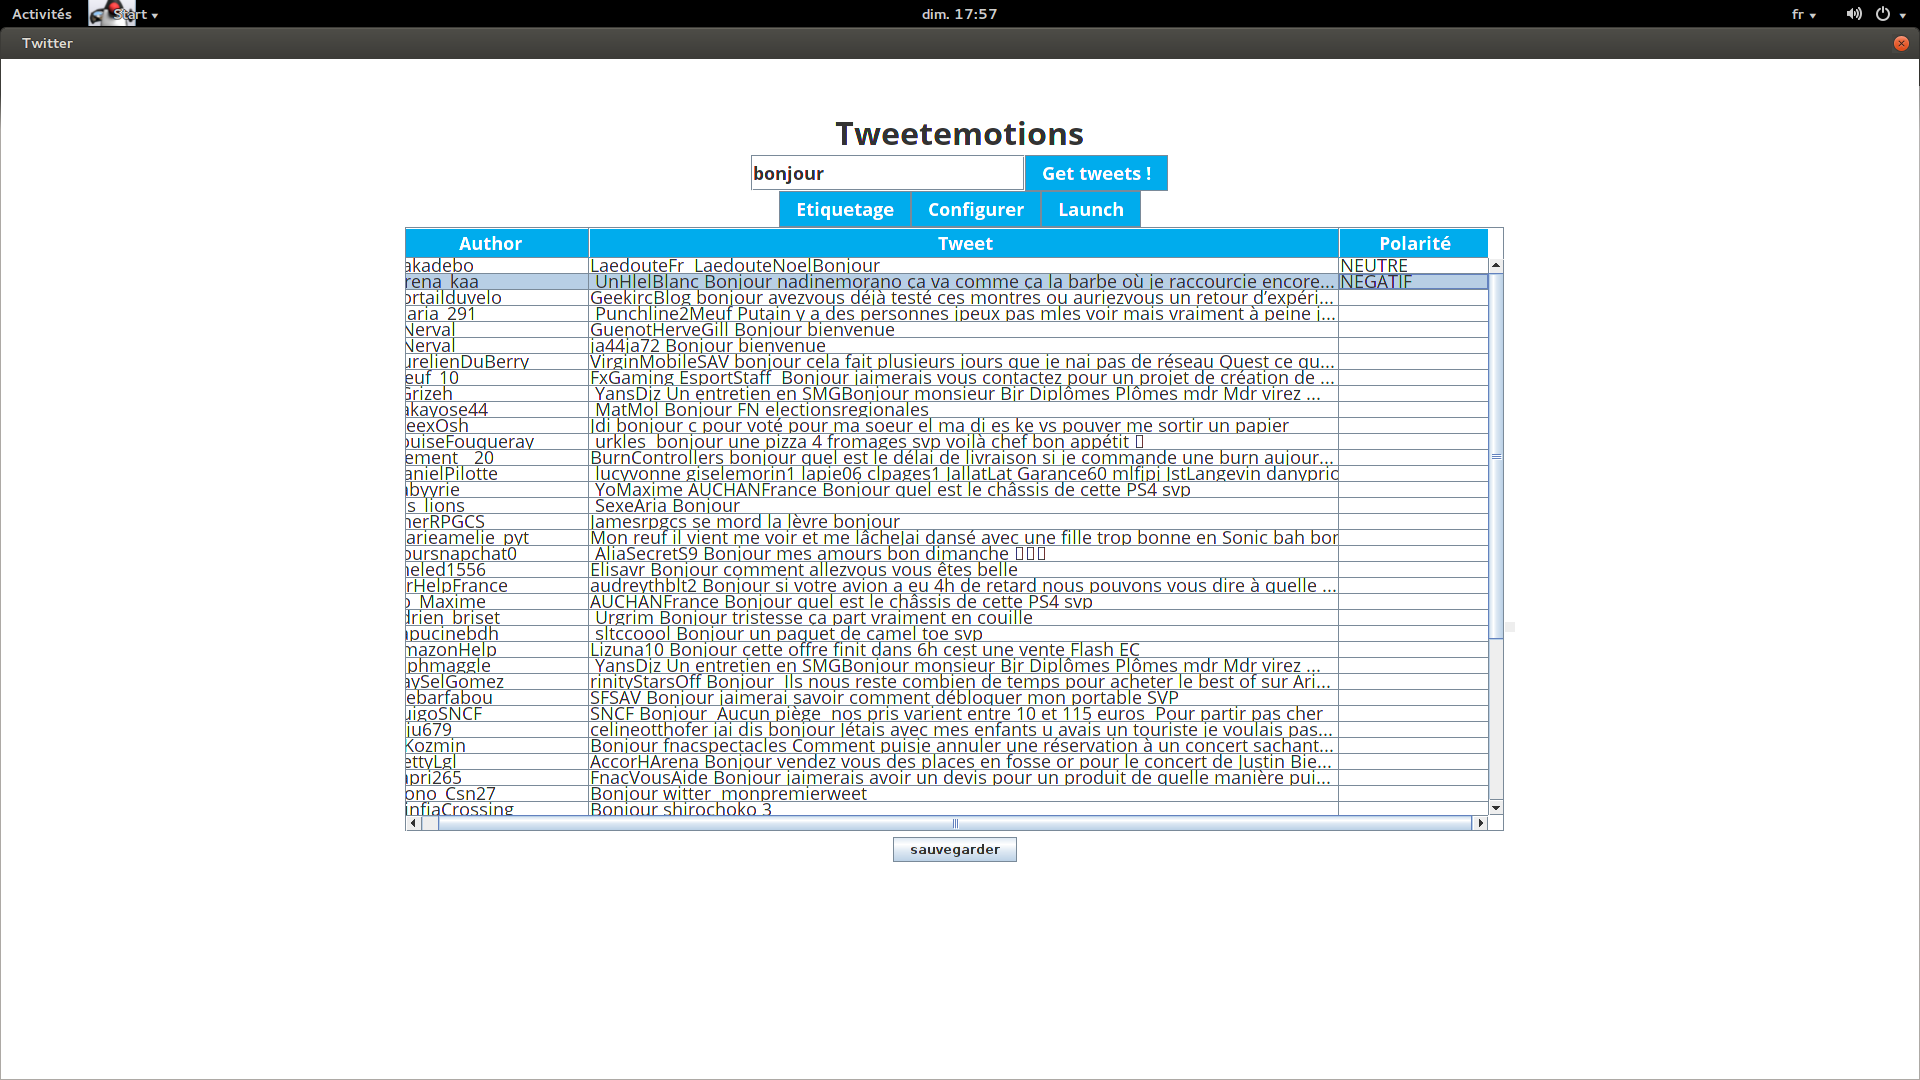
\includegraphics[scale=0.2]{impressions-ecran/etiquetage.png}
	\caption{Étiquetage des tweets}
	\label{etiquetage}
      \end{figure}
      \begin{figure}[H]
	\centering
	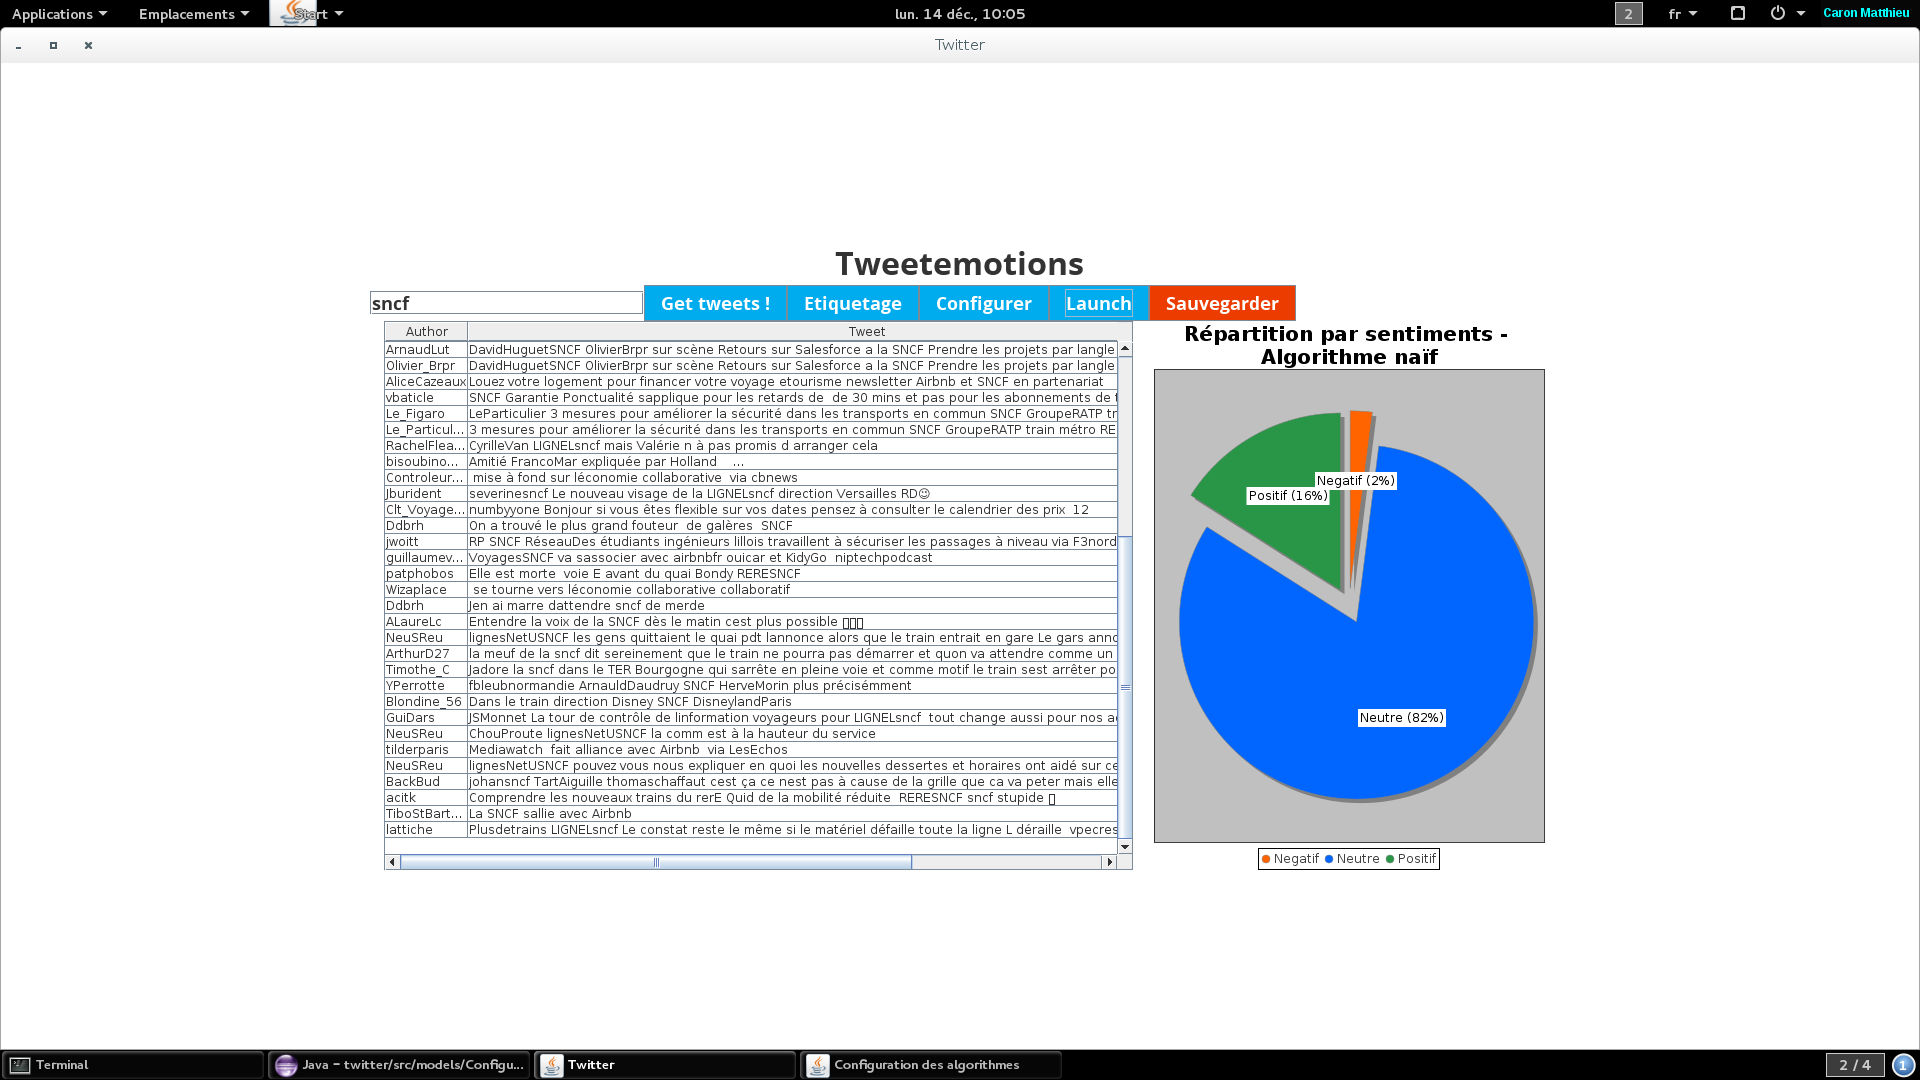
\includegraphics[scale=0.2]{impressions-ecran/dico.png}
	\caption{Algorithme naif}
	\label{dico}
      \end{figure}
      \begin{figure}[H]
	\centering
	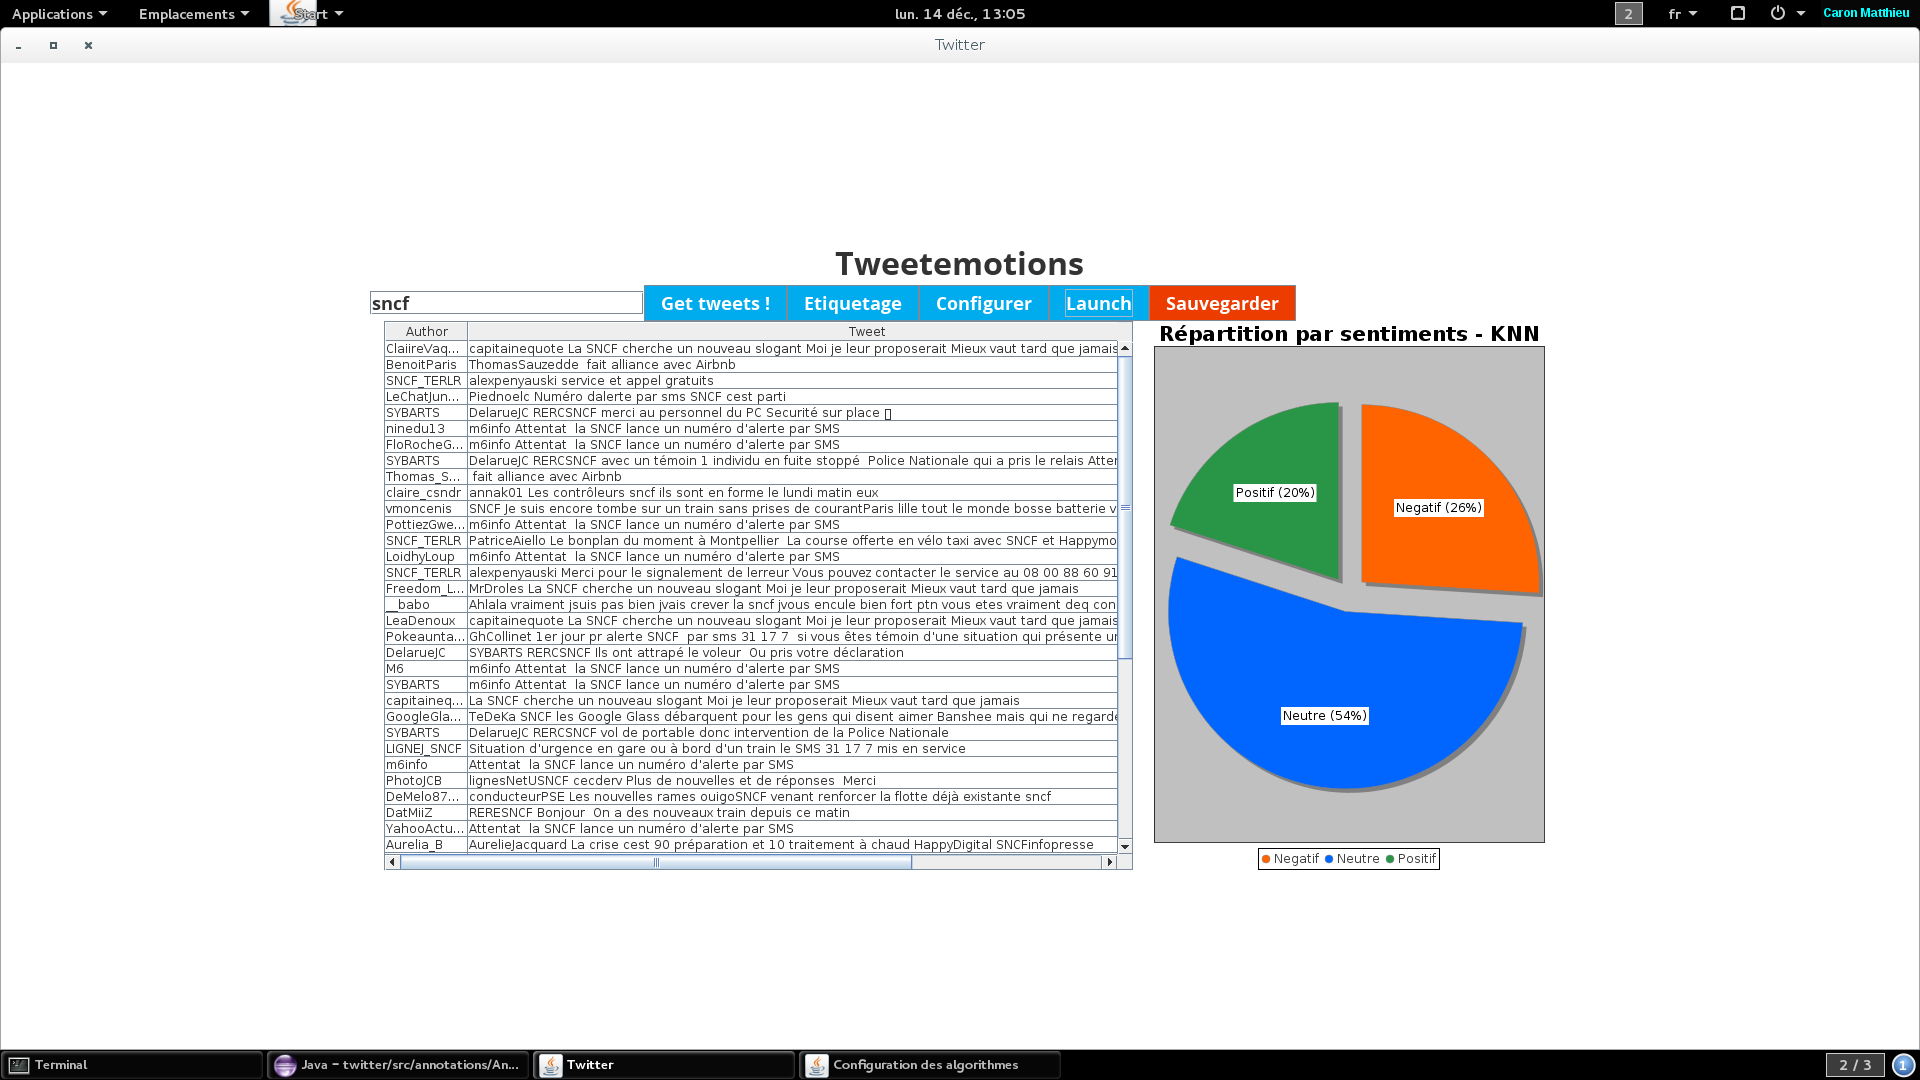
\includegraphics[scale=0.2]{impressions-ecran/KNN.png}
	\caption{Algorithme du plus proche voisin}
	\label{KNN}
      \end{figure}
      \begin{figure}[H]
	\centering
	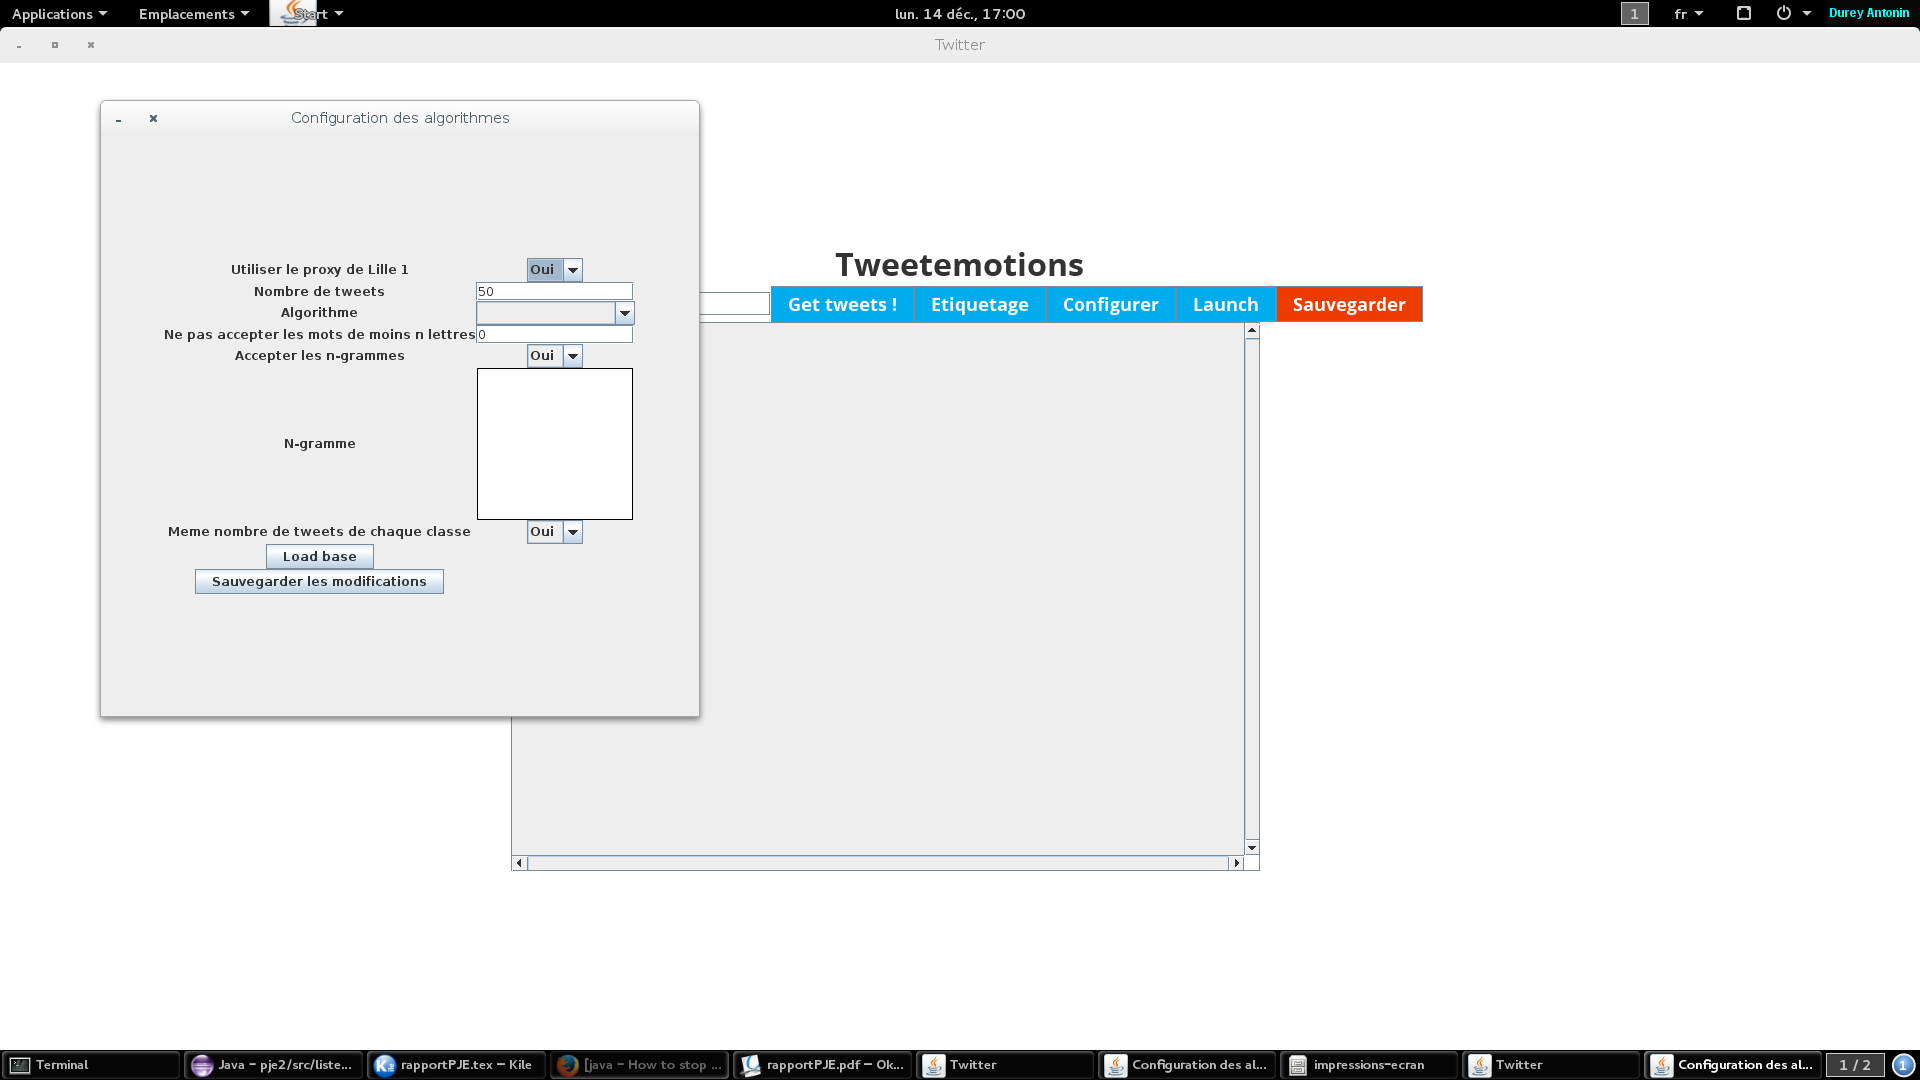
\includegraphics[scale=0.2]{impressions-ecran/config.png}
	\caption{Algorithme du plus proche voisin}
	\label{config}
      \end{figure}
      

    
    \subsection{manuel d'utilisation}
      On lance l'application, la fenetre principale est composée d'un champ de texte, et de boutons \textit{get tweets}, \textit{Etiquettage}, \textit{Configurer} et 
      \textit{Launch}.
      \subsubsection{Le bouton \textit{Get Tweets}}
	Si vous cliquez sur le bouton ``Get Tweets'', l'application va vous demander combien de tweets vous souhaitez récupérer. Une fois le nombre de tweet choisit,
	il va chercher les tweets contenant la chaine de caractère écrite au préalable dans le champ de texte et va afficher ces tweets à l'écran.
	À partir de ce moment tous les calculs (dico, knn et bayes) se feront sur ces tweets.
      \subsubsection{Le bouton \textit{Etiquetage}}
	Ce bouton est utile pour ajouter des tweets à une base de données, il faut avoir au préalable cherché des tweets avec le bouton \textit{Get Tweets}.
	A côté de chaque tweet, il faut choisir quelle est leur polarité : neutre, positif ou négatif \ref{etiquetage}. Une fois ceci fait pour tous les tweets,
	il est possible de sauvegarder les tweets étiquetés. Pour la sauvegarde, un sélecteur de fichiers s'ouvre et 2 choix s'offrent à vous :
	Sauvegarder dans un fichier déjà existant, les tweets seront alors ajoutés au modèle précédemment sauvegardé.
	Sauvegarder dans un nouveau fichier.  
	Dans les 2 cas, il est préférable de choisir un fichier avec l'extension .base puisque c'est ce que nous avons commencé à faire dans notre application.
      \subsubsection{Le bouton \textit{Configurer}}
	Ce bouton sert à configurer l'application. Les options suivantes sont configurables :
	\begin{itemize}
	 \item Utilisation ou non du proxy Lille 1
	 \item Nombre de tweets à récupérer à chaque appel de \textit{Get tweets}
	 \item Utilisation d'une base de tweets équilibrée (nb positifs = nb negatifs = nb neutres)
	 \item Algorithme à lancer sur les tweets obtenus
	 \item Uniquement pour Bayes : ne pas accepter les mots de moins de \textit{n} lettres
	 \item Uniquement pour Bayes : prendre en compte les n-gramme insérés ci-dessous
	 \item Uniquement pour Bayes : les n-grammes, séparés par des virgules. Attention, comme nous avons retiré tout signe de ponctuation, \textit{à l'heure} doit s'écrire \textit{à lheure}.
	 \item Le bouton \textit{Load base} sert à charger la base voulue. La base est stockée sous forme d'objet dans les fichiers comportant l'extension \textit{.base}
	\end{itemize}
	Il est important de sauvegarder les modifications avec le bouton associé, sans quoi celles-ci ne seraient pas prises en compte.
	\ref{config}
\chapter{Résultats de la classification avec les différentes méthodes et analyse}
    \subsection{mots clefs}
      Après analyse, nous avons constaté que 64\% des tweets étaient classés correctement par l'algorithme des mots clefs.
      Pour ce qui est du temps de calcul : 8ms pour 100 tweets. 
    \subsection{KNN}
      Pour Knn, sur 95 tweets différents on a 61\% des tweets classés correctement.
      Pour ce qui est du temps de calcul 442ms pour 100 tweets.
    \subsection{Bayes}
      Pour faire fonctionner bayes il faut que la difference du nombre de mots par classe soit négligeable, pendant qu'on a fait les test on avait la classe neutre qui comportait
      beaucoup trop de tweets, on a donc tronqué notre base pour obtenir un meme nombre de tweet pour chaque classe, le resultat était légerement plus cohérent mais pas satisfaisant
      nous avions donc tenté d'équilibrer à la main et nous nous sommes rendu compte que pour obtenir un résultat cohérent il fallait un nombre de mots quasi équivalent pour chaque classe.
    
    
\chapter{Conclusions}
Suite a nos experimentations, nous pouvons conclure que l'algorithme de mots clefs à l'avantage d'être efficace en temps pour une bonne classification de 64\%
presque autant que KNN.
Il faut prendre les resultats des sondages de sentiments avec des pincettes, puisque la réponse affichée à l'écran ne répond pas à 
est-ce que les gens sont pour ou contre tel sujet, mais plutot combien de tweets contenant tel sujet sont positif ou negatif.
Une autre difficulté dans la classification de tweets, c est le sarcasme, si le sarcasme n'existait pas, la classification serait plus efficace...
Enfin il faut savoir qu'il existe beaucoup de comptes parodiques sur twitter, pour être plus puissant il faudrait ne pas se limiter à juste observer le tweet mais
aussi observer le comptes de la personne qui envoie le tweet pour savoir si elle est plutot serieuse ou pas.



\end{document}     
